
The study of the structure of the proton and other hadrons is a central pursuit in nuclear physics. Since the 1950s, probing this structure has revealed new aspects of nature and ultimately led to the development of the Standard Model. The pioneering experiments of Hofstadter revealed the charge distribution of the proton and nuclei, while the deep-inelastic scatting (DIS) experiments by Kendall, Taylor and Friedman at SLAC and those that followed led to the development of QCD and have mapped out  the distributions of fundamental partonic (quark and gluon) degrees of freedom in the proton. At present, these studies are being complemented by new generations of experiments such as those at the 12 GeV upgrade of Jefferson Lab and a potential Electron-Ion Collider (EIC) that seek to map out the three-dimensional structure of the proton by determining generalized parton distributions and transverse-momentum dependent parton distributions. 

Lattice QCD studies of hadron structure were pioneered in the 1980s and have matured significantly. They are now of a maturity where  rigorous connection to experiment is possible and the prospect of future calculations that will support and complement modern experimental investigations is exciting.


\subsection{Charges, radii,  electroweak form factors and polarizabilities}

The simplest aspects of hadron structure that are probed in electroweak interactions are the various static ``charges'' and moments corresponding to the coupling of bilinear quark currents to the hadron. Generalising to currents involving momentum transfer leads to the  electroweak form factors, with the small momentum behaviour characterized by the electromagnetic and weak radii that correspond to the slopes of the appropriate form factors at zero momentum transfer. These quantities can be determined from LQCD by calculating ratios of three-point and two point correlations functions built from hadronic interpolating operators and quark current operators. This is by now a well-developed approach with various groups around the world presenting results that are close to controlling all systematic uncertainties. Over the next few years, these systematic uncertainties will be further reduced  and  precision will be increased by performing high statistics calculations with additional lattice spacings and volumes. In addition, the full flavor-dependence of the moments, radii and form factors will be determined. 

There are a number of particularly important cases in this class of LQCD calculations. 
\begin{itemize}
	\item The axial charge of the nucleon is a benchmark quantity that is known very precisely from experiment, $g_A=1.2723(23)$ \cite{Patrignani:2016xqp}. LQCD calculations are also becoming more precise, with uncertainties at the few percent level  \cite{Bhattacharya:2016zcn,Yoon:2016jzj,Chang:2018uxx,Gupta:2018qil}. With the significant increase in precision that will occur in the next few years, it is possible that this will  become a quantity that tests the Standard Model; this is particularly relevant in the context of current anomalies in different measurements of the neutron lifetime. Recent calculations of this quantity by USQCD collaboration members are becoming increasingly precise.
	
	\item The scalar charge of the nucleon dictates the sensitivity of searches for important classes of dark matter candidates at direct-detection experiments. Along with the tensor charge \cite{Gupta:2018lvp}, the scalar charge \cite{Shanahan:2016pla}  is also relevant theory input to other searches for physics beyond the Standard Model. These quantities are discussed further in the companion white paper on Fundamental Symmetries \cite{wpfund}.
	
	\item The proton charge radius is  of significant phenomenological interest as there are very significant discrepancies in its extraction from muonic hydrogen spectroscopy  and from electronic hydrogen spectroscopy and electron-proton scattering. Existing LQCD calculations of the isovector charge radius of the
proton~\cite{Capitani:2015sba,Hasan:2017wwt,Alexandrou:2017ypw,Ishikawa:2018rew,Detmold:2018ptb,Alexandrou:2018sjm}  have $\sim10$\% precision, assigning conservative estimates of the systematic uncertainties that are not well-quantified. A  percent-level  LQCD calculation of the isovector radius combined with existing precise measurements of the charge radius of the neutron are sufficient to determine the proton charge radius at a level where LQCD calculations will  have impact on the discrepancy. 
	
	\item The axial current form factors of the nucleon and nuclei are relevant for neutrino physics as discussed extensively in the  accompanying whitepaper on lattice QCD for neutrino physics \cite{wpneutrino}.
\end{itemize} 
These quantities are relatively simple to calculate  and have been analyzed by the community in Ref.~\cite{Lin:2017snn} and  are being included in the upcoming 2018 Flavor Lattice Averaging Group (FLAG {\tt http://flag.unibe.ch})
review of LQCD calculations.

Second order responses to EM fields are quantified by the electric and magnetic (and higher-order spin) polarizabilities of hadrons. LQCD calculations of polarizabilities have used spectroscopy in fixed external fields~\cite{Detmold:2006vu,Detmold:2009dx,Detmold:2010ts,Freeman:2014kka,Lujan:2014kia,Chang:2015qxa,Lujan:2016ffj,Shanahan:2017bgi,Tiburzi:2017iux} or direct measurement of hadronic four point functions corresponding to two current insertions~\cite{Engelhardt:2007ub}. Being somewhat complicated observables, polarizability calculations with close to physical quark masses and with explicit control of all systematic uncertainties are lacking but will be possible with the levels of resources available in the next five years.

\subsection{Parton Distribution Functions}

The DIS experiments begun at SLAC in the late 1960s, led the way to the observation of asymptotic freedom and the development of QCD as a non-Abelian gauge theory. Efforts to better determine the partonic structure seen inside the proton have continued ever since. The parton distributions functions (PDFs), which quantify the densities of quarks and gluons in a hadron as a function of the longitudinal momentum fraction, $x$, are important inputs for experiments at hadron colliders such as the LHC and must be better constrained to fully exploit these experimental programs.
They  are defined by matrix elements in a hadron state of bi-local operators separated along the light-cone and are intrinsically difficult to access from LQCD calculations in Euclidean space ~\cite{Collins:1981uw,Curci:1980uw,Baulieu:1979mr,Collins:1989gx} .


\subsubsection{Moments of Parton Distribution Functions}

The most well-established computations that address the partonic structure of hadrons are based on calculations of matrix elements of the local twist-two operators that arise in the light-cone operator product expansion (OPE) of DIS and related processes. These matrix elements determine the Mellin moments of the underlying parton distributions; with  a sufficient number of moments the PDF can be reconstructed with controlled uncertainties. However, the reduced symmetries of the spacetime lattice used in LQCD calculations (typically, the hypercubic group H(4)) compared to the Lorentz group means that the OPE is complicated by divergent mixing between operators.
Lattice operators corresponding to the lowest few moments of the unpolarized, polarized and transversity distributions can be chosen such that this mixing is absent at the expense of having nonzero matrix elements only in states of nonzero three-momentum. LQCD calculations of these matrix elements have been undertaken since the first calculations of Martinelli and Sachrajda \cite{Dawson:1997ic} in the 1980s. A recent summary of the calculations of PDF moments is given in \cite{Lin:2017snn}.
	
To go beyond the lowest moments, operators involving more complicated finite difference discretizations of the derivative operators can be constructed following ideas developed in Ref.~\cite{Davoudi:2012ya} for  three-dimensional discretizations of interpolating operators of fixed angular momentum. By using multiple copies of given irreducible H(4) representations (irreps), better approximations to operators transforming irreducibly under SO(4) symmetries can be constructed. This approach is being actively investigated at present \cite{IDavoudiLattice2018} and offers the possibility of calculations of sufficient numbers of moments that a parameterization of the underlying PDF can be constrained.



\subsubsection{Quasi-distributions and pseudo-distributions}



The formulation of lattice QCD in Euclidean space severely restricts
lattice calculations of partonic structure.  
The analytic continuation of the matrix elements that define the PDFs to Euclidean space is highly non-trivial due to the fact that these matrix elements are not local in time. Recently, new ideas,  known as the "Large Momentum Effective Field Theory" (LaMET),  have
been proposed that aim to circumvent this problem~\cite{Ji:2013dva,Ji:2014gla}.
In this approach, one computes a time local version of the matrix element that defines the PDF in Euclidean space
where the external states have a suitably large momentum  and the
bi-local quark insertion is separated by some spatial distance.
%
With these choices, the quasi-PDF is defined by the Fourier transform over the spatial extent of the equal-time matrix element of a spatially directed Wilson-line between quark fields, at some lattice scale. To relate this lattice quasi-PDF to the desired Minkowski light-cone PDF, matching conditions are implemented within the LaMET~\cite{Ji:2013dva,Ji:2014gla} scheme after either perturbative or non-perturbative~\cite{Martinelli:1994ty} renromalization. Power corrections that break the matching  procedure from  higher-twist effects are suppressed at large nucleon momentum. This approach has been recently used  for quasi-PDFs  in Refs.~\cite{Alexandrou:2017huk,Chen:2017mzz,Green:2017xeu,Chen:2018xof,Lin:2018qky}. A recent determination of the isovector unpolarized and polarized PDFs of the  nucleon is shown in Figure~\ref{fig_quasipdf}.

\begin{figure}[h!]
	\centering
	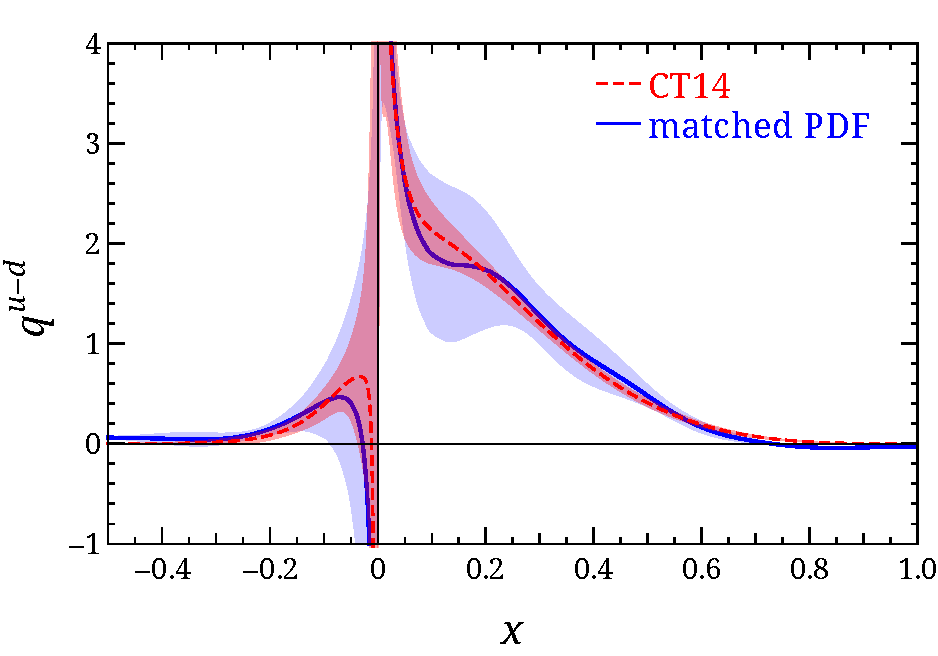
\includegraphics[width=0.45\columnwidth]{figures/LP3-PDF-CT14}\hspace{1cm}
	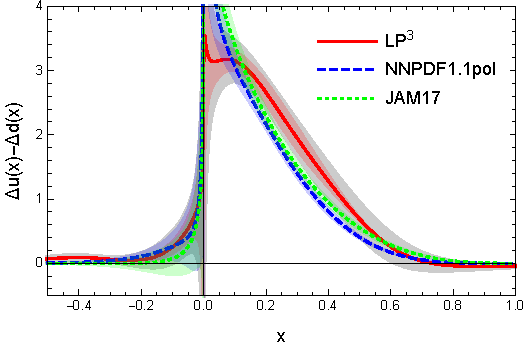
\includegraphics[width=0.45\columnwidth]{figures/a09m130-helicity-comp}
	\caption{Left: Unpolarized isovector nucleon PDF with comparison to the CTEQ parameterization~\cite{Chen:2018xof}.
		Right: Polarized isovector nucleon PDF with comparison to the NNPDF parameterization~\cite{Lin:2018qky}.}
	\label{fig_quasipdf}
\end{figure}


An alternative approach, named the pseudo-PDF, considers the ratio of the equal time matrix element of the Wilson line between quarks with the rest-frame density matrix element. The equal time matrix element is parameterized in terms of the product of the spatial momentum with the spatial separation forming a Lorentz invariant called the Ioffe time~\cite{Ioffe:1969kf,Braun:1994jq}, and the ratio corresponds to the Ioffe time distribution~\cite{Radyushkin:2016hsy,Radyushkin:2017cyf}.
%
This ratio is free of UV divergences and requires no renormalization. The key distinction between the quasi and pseudo PDF approaches is that in the latter the Fourier transform over all spatial separations is not, in practice, needed. Indeed, recent work has shown that there can be large finite-volume effects within the spatial integration~\cite{Briceno:2018lfj}. An observation from initial lattice calculations using the pseudo-PDF approach~\cite{Karpie:2018zaz,Karpie:2018zaz}  is that Ioffe-time distributions exhibit factorization down to small distances in the spatial separation, where the small distance behavior of the pseudo-PDF  satisfies a perturbative  evolution equation. Thus, rather than computing the entire PDF as a function of Bjorken-$x$, the PDF is parameterized as a function of $x$, similar to approaches taken in phenomenological studies~\cite{Ball:2017nwa,Accardi:2016qay}. Larger lattice sizes with smaller lattice spacing will allow for better probes of the perturbative evolution scale, and better constraint of the small-$x$ region.

\subsubsection{Good lattice cross sections}
Analogous to extracting PDFs from QCD global fits of high energy scattering data, PDFs can also be extracted from analyzing ``data'' generated by LQCD calculation of good {\it lattice cross sections} \cite{Ma:2014jla,Ma:2014jga}. A {\it lattice cross section} is defined in Refs.~\cite{ Ma:2014jla,Ma:2014jga} as a single-hadron matrix element of a time-ordered, renormalized nonlocal operator ${\cal O}_n(z)$: ${\sigma}_{n}(\nu,z^2,p^2)=\langle p| {T}\{{\cal O}_n({z})\}|p\rangle$ with four-vector momentum, $p$, antiquark quark-pair separation $z$, and $\nu\equiv p\cdot z$. The values of $p$ and $z$, and the choice of ${\cal O}_n$, determine the dynamical features of the lattice cross section. A useful lattice cross section should have the following three key properties: (1) calculable in LQCD in Euclidean time, (2) has a well-defined continuum limit as the lattice spacing $a\to 0$, and (3) has the same factorizable logarithmic collinear divergences as that of PDFs, which connects the good lattice cross sections to PDFs, just as high energy hadronic cross sections are related to PDFs in terms of QCD factorization.  

A class of { good} lattice cross sections was constructed in terms of a correlation of the product of two {renormalizable} currents (see also the following subsection).  There are many possible choices for the current, such as a vector quark current, or a tensor gluonic current~\cite{Ma:2017pxb}.  Different combinations of the two currents help enhance the lattice cross sections' flavor dependence.  If spatial separation between the currents is sufficiently small, the lattice cross section constructed from two renormalizable currents can be factorized into PDFs and perturbative hard kernels \cite{Ma:2017pxb},
and the PDFs can be extracted from global fits of lattice-QCD generated data for various lattice cross sections $\sigma_{n}(\nu,z^2,p^2)$ with corresponding perturbatively calculated coefficients.

The quasi-PDFs and pseudo-PDFs introduced above are derived from choosing a single anti-quark quark pair separated in space by a Wilson line.
With two space separated currents, modulo $O(\alpha_s)$ and higher twist corrections, one finds that a quasi-quark distribution is obtained when a cross-section is computed for fixed momenta, while the pseudo-quark distribution is object if the cross-section is computed with fixed spatial separation of the currents.  
That is, these two approaches for extracting PDFs are equivalent if matching coefficients are calculated at the lowest order in $\alpha_s$ neglecting all power corrections, but different if contributions from either higher order in $\alpha_s$ or higher powers in $z^2$ are considered.

\subsubsection{Hadronic tensor methods}

A variety of other approaches are also being investigated to access hadronic structure based on computations of the hadronic tensor \cite{Liu:1993cv,Aglietti:1998mz,Detmold:2005gg,Liu:2016djw}. In the first of these approaches \cite{Liu:1993cv,Liu:2016djw}, partonic physics is accessed through a discrete Laplace transform of the Euclidean hadronic tensor. Various implementations of the challenging inverse problem that is involved have been investigated in \cite{Liang:2017mye}. In the second approach, a fictitious heavy quark field is introduced and the corresponding hadronic tensor involving heavy-light currents and resulting lattice correlation functions are matched on to the relevant OPE to extract the moments of regular parton distributions. This approach requires very fine discretization scales, but first investigations are now beginning \cite{Detmold:2018kwu}. 
An additional approach based on transforms of the hadronic tensor is being pursued in Refs.~\cite{Chambers:2017dov}.

\subsection{Generalized Parton Distribution Functions}

Generalized parton distributions (GPDs) \cite{Ji:2001wha,Radyushkin:1997ki,Diehl:2003ny,Belitsky:2005qn} provide further insight into the quark and gluon structure of hadrons, combining parton dependence on longitudinal and transverse position (when viewed in their impact-parameter space formulation \cite{Burkardt:2000za}). GPDs are defined as  off-forward matrix elements of the same operators that define parton distributions.   Information about GPDs is accessible from deeply virtual Compton scattering and deeply-virtual vector meson production in particular. Basic aspects of these distributions have been investigated at JLab, COMPASS and HERMES and a significant fraction of the experimental program at the 12GeV upgrade of Jefferson Lab is focused on revealing more  information about  GPDs. Lattice calculations have focused on the generalized form factors (GFFs) that parametrize off-forward matrix elements of local twist-two operators and correspond to moments of GPDs \cite{Hagler:2003jd,Hagler:2007xi,Hagler:2009mb}. 

For the unpolarized case
GPDs also encode the spin decomposition of the proton through Ji's sum rule \cite{Ji:1996ek} that separates quark spin, orbital angular momentum and the total gluon angular momentum. 
A further decomposition, known as the Jaffe-Manohar decomposition \cite{Jaffe:1989jz}, is valid in light-cone gauge. These decompositions of the proton spin has recently been investigated in Refs.~\cite{Yang:2016plb,Alexandrou:2017oeh}.
The $n=2$ GFFs  parameterize the matrix elements of the energy momentum tensor. As well as determining the momentum distribution and spin, they 
also define the pressure and shear distributions in the hadron~\cite{Polyakov:2018zvc}.

The first calculations of the quark GFFs for $n=2,3$ were performed by USQCD collaboration members \cite{Hagler:2003jd} with many subsequent improvements (see Ref.~\cite{Hagler:2009mb} for a review). The isovector combination of the unpolarized and polarized GFFs have been studied at quark masses corresponding to $m_\pi>200$ MeV, but not yet at the physical point \cite{Syritsyn:2011vk,Bali:2013dpa,Hagler:2007xi,Bratt:2010jn,Sternbeck:2012rw,Brommel:2007sb,Gockeler:2003jfa,Alexandrou:2011nr}. In most calculations of the isoscalar GFFs, the disconnected contractions have been omitted with the notable exception of Ref.~\cite{Deka:2013zha}, and mixing of the quark operators with gluon operators has been ignored given the small size of perturbative mixing coefficients \cite{Alexandrou:2016ekb}.  Calculations in the next few years will address these quantities with high fidelity, controlling all systematic uncertainties.


\subsection{Transverse momentum-dependent parton distributions}
\label{TMDs}

Transverse momentum-dependent parton distributions  \cite{Boer:2011fh} (TMDs)
constitute one of the pillars on which the three-dimensional tomography of
hadrons rests. Together with the three dimensional spatial information
derived from GPDs, they permit a comprehensive reconstruction of hadron substructure and thus
encode orbital angular momentum contributions to nucleon spin, and
spin-orbit correlations in hadrons. Through the selection of
particular parton spin and transverse momentum components, a
variety of TMDs can be probed, including naively time-reversal odd
(T-odd) quantities such as the Sivers and Boer-Mulders functions.
These latter TMDs exist by virtue of initial or final state interactions
in corresponding physical processes, introducing a preferred chronology
in the description of the process.

In view of the fundamental importance of TMDs and the rich spectrum of
effects that can be probed, TMDs have been, and continue to be the
target of a variety of experimental efforts. Deep-inelastic scattering
experiments performed by COMPASS \cite{Alekseev:2008aa,Adolph:2014fjw},
HERMES \cite{Airapetian:2009ae,Airapetian:2013bim} and Jefferson Lab
\cite{Qian:2011py,Avakian:2010ae} have yielded TMD data including evidence
for the T-odd Sivers effect. Complementary Drell-Yan experiments at
COMPASS \cite{Gautheron:2010wva} and Fermilab \cite{Brown:2014sea} are
envisaged, which could, in particular, test the sign change between
the SIDIS and DY processes. Related transverse single-spin
asymmetries have been measured at RHIC in polarized proton-proton
collisions \cite{Adare:2013ekj,Adamczyk:2012xd}. Further experimental
efforts at RHIC are projected to provide insight into strong QCD evolution
effects expected for the Sivers TMD \cite{Echevarria:2014vda}.
TMDs furthermore constitute a central focus of the proposed Electron-Ion
Collider facility \cite{Accardi:2012qut}.

\begin{figure}
	\centering
	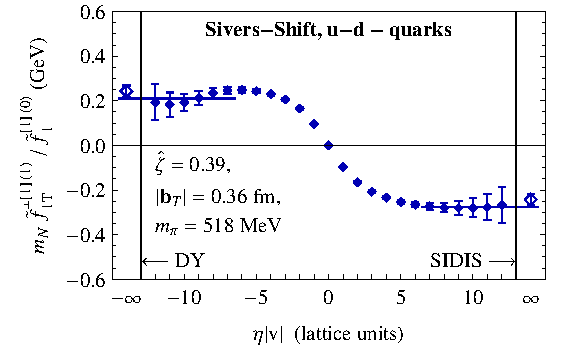
\includegraphics[width=0.95\columnwidth]{figures/m020_run38_UminusD_Sivers_lsqr-9_zetasqrlat4}\hspace{1cm}
	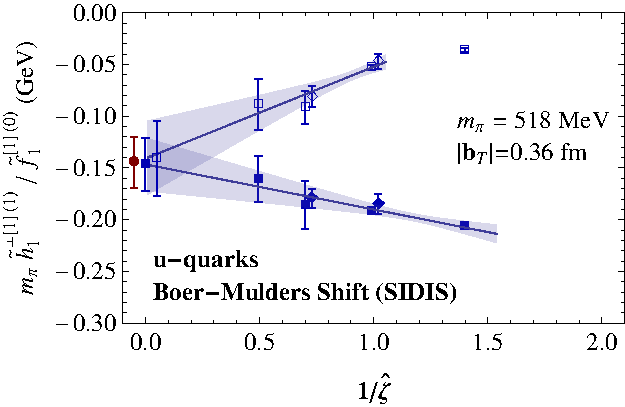
\includegraphics[width=0.95\columnwidth]{figures/new_bm_u_sidis_b0p36_vszetahat_extrap_pow1}
	\caption{Top: Proton Sivers shift as a function of staple length, $\eta$, for fixed
		staple width, $b_T, $ and rapidity (Collins-Soper) parameter, $\hat{\zeta }$;
		$\eta \rightarrow \infty $ defines the SIDIS limit \cite{Musch:2011er}.
		Bottom: Extrapolation of the SIDIS limit data for the pion Boer-Mulders
		shift to the physical limit of large $\hat{\zeta }$
		at fixed $b_T $ \cite{Engelhardt:2015xja}. Open symbols represent a partial
		contribution that dominates at large $\hat{\zeta } $, providing further
		insight into the approach to the asymptotic regime.}
	\label{fig_sidis}
\end{figure}

To complement and support these efforts, a sustained
project to calculate TMD observables within LQCD was initiated
and developed by USQCD collab members and their collaborators in Refs.~\cite{Hagler:2009mb,Musch:2010ka,Musch:2011er,Engelhardt:2015xja,Yoon:2017qzo,Engelhardt:2017miy}.
TMDs are formally defined through matrix elements of a bilocal quark
operator in which the quark fields are connected through a gauge link
along a staple-shaped path. Building on the preliminary investigations of Refs.~\cite{Hagler:2009mb,Musch:2010ka}, the first full calculation of TMD
observables using staple-shaped gauge links was performed in
\cite{Musch:2011er}, obtaining results on the Sivers and Boer-Mulders
shifts, a worm-gear shift, and the generalized transversity.
Fig.~\ref{fig_sidis} (left) displays a  result for the Sivers
shift, exhibiting its T-odd character and the SIDIS and DY limits
achieved for asymptotic staple lengths.

Such lattice TMD calculations face several challenges. One such challenge is achieving
the  limit of large rapidity difference between between struck
quark and hadron remnant in a deep inelastic scattering process, which
is encoded in the space-time direction of the staple link. An investigation
of the Boer-Mulders shift in a pion dedicated to elucidating this limit
was reported in Ref.~\cite{Engelhardt:2015xja}. A result from this study is
shown in Fig.~\ref{fig_sidis} (right), demonstrating access to the large
rapidity regime. Another challenge is understanding renormalization,
operator mixing and scaling. Observables such as the Sivers shift are
constructed as ratios in which certain renormalization factors cancel
in continuum QCD; to test whether this pattern persists in the lattice
formulation, a comparison between TMD calculations on clover and domain
wall fermion ensembles at approximately the same pion mass was performed
and reported in Ref.~\cite{Yoon:2017qzo}, corroborating the cancellation of 
renormalization factors expected from continuum QCD.
On the other hand,
in the case of the worm-gear shift, operator mixing is predicted for
clover fermions \cite{Constantinou:2017sej}, which destroys the simple
cancellation in ratios; evidence for this was also seen in the data
collected in \cite{Yoon:2017qzo}.
A preliminary study~\cite{Engelhardt:2015czw} with nearly physical
pions indicates that higher statistical precision is required to impact phenomenology. New efforts
that will be undertaken over the next few years include the use of boosted nucleon sources to access the large
rapidity regime, as well as excited state control through calculation
for a range of source-sink separations.

In addition to the aforementioned calculations, which concentrated on
transverse momentum dependence while integrating over longitudinal
momentum fraction $x$, there are explorations of the
$x$-dependence of the Sivers shift, achieved by adding a
longitudinal separation in the bilocal quark operator defining TMDs.
Furthermore, the generalization
of TMDs to non-zero momentum transfer (GTMDs) was explored in
Ref.~\cite{Engelhardt:2017miy}, with a specific focus on the direct
calculation of quark orbital angular momentum (OAM) in the proton.
Considering non-zero momentum transfer supplements the transverse
momentum information with transverse position information, thus
yielding direct information on OAM (as opposed to indirect access
as $L=J-S$ via Ji's sum rule). Moreover, this approach allows one
to not only determine the Ji OAM, but also the Jaffe-Manohar OAM.

{\it TMDs: Future opportunities:}

The investigations described above provide the necessary foundation for
the controlled, precise prediction of selected TMD observables from
lattice QCD. The chief systematic challenges have been explored,
and a tentative roadmap of incremental refinement of the calculations can
be projected. The use of boosted nucleon sources will allow access to the large
rapidity regime. Discretization effects will need to be quantified
as momenta are increased. This, as well as a quantitative treatment
of the renormalization and QCD evolution of lattice TMD observables,
building on the initial study of Ref.~\cite{Yoon:2017qzo} will necessitate a
sequence of calculations with decreasing lattice spacings.

In assessing the required resources for this program, it should be noted that lattice
TMD calculations are dominated by the cost of the large number of
contractions, as opposed to the cost of the inversions needed to
obtain propagators. The large number of contractions results from the multitude of
staple-shaped gauge link geometries that must be surveyed in order
to perform the necessary extrapolations to long staple length as
well as large rapidity difference between struck quark and hadron
remnant in a deep-inelastic scattering process. 

A further aspect that remains to addressed is the flavor separation
of TMD observables and sea quark effects, as targeted, e.g., by the Fermilab
E-906/SeaQuest experiment. This calls for the evaluation of disconnected
diagram contributions, which hitherto have not been studied in lattice TMD
investigations. Efficient calculation of these diagrams will be possible
with the use of hierarchical probing methods \cite{Stathopoulos:2013aci}.
Future calculations will also need to account for mixing of gluonic
operators with flavor singlet quark operators, which have not been considered.

Besides these improvements of the systematics of lattice TMD
calculations,  the incorporation of further physics objectives is
also planned. To date, calculations have focused on transverse nucleon
polarization, with which one can probe the particularly interesting
Sivers and Boer-Mulders effects. Nonetheless,  the TMDs associated
with longitudinal nucleon polarization are also of interest and include a
second worm-gear function in addition to the one probed with transverse
polarization. TMD calculations with longitudinal polarization are
straightforward to implement in the existing scheme. Furthermore, the
extension of lattice calculations to include the $x$-dependence of TMDs,
already explored for the case of the Sivers shift as noted above, must be
continued to encompass a variety of TMD observables.

In addition, the study of GTMDs, i.e., TMDs in the presence of a
momentum transfer, must be extended beyond the specific case of quark
orbital angular momentum \cite{Engelhardt:2017miy}. For example, spin-orbit correlations of quarks
in the proton can be quantified through the GTMD $G_{11} $ in the
classification scheme of Ref.~\cite{Meissner:2009ww}.
Complementary ways of accessing quark orbital
momentum, e.g., through the twist-3 GTMDs $F_{27} $, $F_{28} $, related
to the GPD $\widetilde{E}_{2T} $, will also be explored  \cite{Meissner:2009ww}.




\subsection{Gluon aspects of hadron structure}

While gluons and the QCD interactions they embody play an essential role in the binding of hadrons, gluon contributions to hadron structure observables are far less well known than their quark analogues. Understanding the role of gluons in hadron structure has become a major goal of experimental facilities, such as COMPASS~\cite{Adare:2014hsq} and STAR~\cite{Djawotho:2013pga}. Furthermore, a primary mission of the proposed Electron-Ion Collider~\cite{Accardi:2012qut,Kalantarians:2014eda}, which is the highest priority for new construction in the NSAC nuclear physics long-range plan~\cite{Geesaman:2015fha}, is to image the gluon structure of hadrons and nuclei. This program will access the three-dimensional gluon structure of the nucleon and allow first measurements of gluon GPDs and TMDs, complimenting significant efforts at RHIC to measure the gluon contribution to the nucleon spin,  potential experiments to study gluon distributions at JLab~\cite{Maxwell:2018gci,Hattawy:2017woc,Dobbs:2017vjw}, and those at the LHC~\cite{Baltz:2007kq}. 
%
In this light, LQCD calculations of gluon structure quantities have taken on renewed importance. There has been significant progress on this front over the last five years~\cite{Alexandrou:2017oeh,Yang:2016plb,Detmold:2016gpy,Detmold:2017oqb,Winter:2017bfs,Alexandrou:2016ekb}, expanding and building on pioneering studies of the unpolarised gluon structure of the pion and nucleon~\cite{Meyer:2007tm,Horsley:2012pz,Alexandrou:2013tfa,Deka:2013zha} over the last decade. 

In particular, LQCD calculations have provided new insight into the proton spin crisis---the realization that quarks carry only a relatively small fraction of the proton spin---with calculations of the key and poorly-known gluon contributions to the nucleon spin \cite{Alexandrou:2017oeh,Yang:2016plb}.  As compared to global analyses of polarized parton distributions \cite{deFlorian:2014yva}, a significantly improved constraint on the total gluon helicity is included in Ref. \cite{Yang:2016plb}. An important component of these studies is the renormalization of the gluonic operators, which is being achieved using  perturbative \cite{Glatzmaier:2014sya,Alexandrou:2017oeh} and non-perturbative~\cite{Yang:2018bft} approaches. Complementing this direction, new understanding of the decompositions of the nucleon spin within LQCD has been achieved, giving interpretation to the   orbital angular momentum~\cite{Engelhardt:2017miy}. 
%
In another impressive success, the gluon contribution to the nucleon's momentum has been resolved at 10\% precision, with the momentum sum rule (including separate determinations of the quark and gluon connected and disconnected contributions) found to be satisfied at quark masses corresponding to the the physical value of the pion mass~\cite{Alexandrou:2017oeh}. Extensions of this work will rival the precision of phenomenological parton distribution fits (e.g., CT14NNLO~\cite{Dulat:2015mca}) in the next few years \cite{Lin:2017snn}.
%
First calculations of some of the moments of the gluon GPDs~\cite{Diehl:2003ny} that describe the distribution of gluons in hadrons both in the transverse plane and in the longitudinal direction~\cite{Detmold:2016gpy,Detmold:2017oqb} have also been performed, providing  insight into details of the three-dimensional gluon structure of hadrons, albeit without full investigation of systematic uncertainties. 
First calculations of the momentum transfer dependence of the gluon energy-momentum tensor form factors as well as the gluon contributions to the pressure and shear distributions in the proton have recently been performed \cite{Shanahan:2018nnv,Shanahan:2018pib} (see Fig.~\ref{gluefig}). These latter calculations have been combined with recent experimental studies of the quark contributions to the pressure \cite{Burkert:2018bqq}, leading to a first complete determination of this fundamental quantity.
Moreover, aspects of the gluon structure of nuclei have been studied for the first time,  as described in Section~\ref{sec:nuclearstructure}.

\begin{figure}
	\centering
	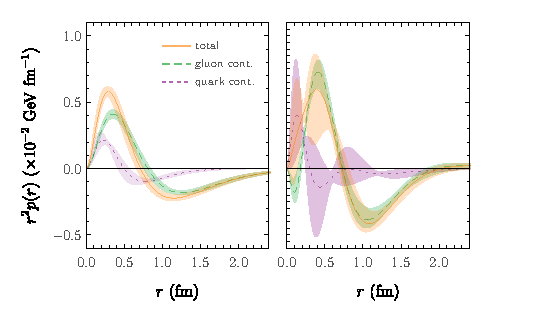
\includegraphics[width=0.95\columnwidth]{figures/combinedpressurelattnew.pdf}
	\caption{The quark and gluon contributions ot the total pressure distribution in the proton from LQCD. Taken from Ref.~\cite{Shanahan:2018pib}. The left panel corresponds to dipole parameterisations, while the right panel corresponds to the more general $z$-parameterisation form.}
	\label{gluefig}
\end{figure}



{\it Gluon structure: future opportunities}

Exascale computing resources and concurrent algorithm development will facilitate LQCD calculations of static gluon structure quantities with controlled statistical and systematic uncertainties. Calculations on  large lattice volumes that become possible with such resources  will achieve significant precision gains through volume averaging and thereby reduce the gauge noise, which is a statistical challenge for calculations of gluon observables. Nevertheless, these studies face large analysis costs and achieving controlled estimates for non-static quantities requires elimination of excited states, and extrapolation to infinite volume as well as to the continuum limit. 
This becomes especially challenging for large nucleon momenta (as required to extract the $x$-dependence of PDFs, GPDs and TMDs) and in the approach to the continuum limit. 
%
In the near term, precise calculations of moments of gluon distributions encoding the contribution of gluons to the mass, momentum, and spin of the nucleon and of other hadrons will be refined. In particular, one can expect calculations at quark masses corresponding to the physical pion mass with fully-controlled uncertainties at the level of 2-5\% precision. To achieve this level of systematic control, it is necessary to precisely determine the renormalization factors, including mixing between the gluon observables and the flavor-singlet quark disconnected terms. This carries significant computational cost in its own right.\\
 

The gluon radius of the nucleon is a quantity as fundamental as the charge radius. Currently, it is not known quantitatively or qualitatively, from experiment or theory, how the charge and gluon radii compare. 
Defined by the slope of the spin-averaged gravitational form factor at zero momentum transfer, the gluon density radius is related via the operator product expansion to matrix elements of the gluon part of the energy-momentum tensor.
The radii and $Q^2$-dependence of the generalized gluon form factors can be calculated using LQCD for both hadrons and light nuclei~\cite{Detmold:2017oqb,Winter:2017bfs}.
On a few-year timescale, fully-controlled calculations of gluon generalized form factors for the nucleon, for low moments and to a scale of several GeV$^2$, can be expected.
From experiment, comparison of nuclear quark and gluon radii will likely be possible through measurements of the parton densities in ${}^4$He at the JLab 12 GeV program~\cite{Hattawy:2017woc}, or from direct measurements of nuclear and nucleon gluon densities using heavy quark production at the planned EIC~\cite{Chudakov:2016otl}. \\

In the longer term, coinciding with the era of sustained exascale computing, one can expect that the $x$-dependence of gluon PDFs and TMDs will be determined from LQCD. Defined on the light-cone, these quantities can not be calculated directly on a Euclidean lattice but can be accessed via rotations to `quasi' or `pseudo' PDFs, matched back to the physical quantities in the large-momentum limit. For the quark PDFs and TMDs these approaches have shown great promise and early success~\cite{Lin:2014zya,Alexandrou:2015rja} (see also Section~\ref{TMDs}). Ultimately, extending these calculations to include gluon distributions will allow a complete decomposition of the three-dimensional quark and gluon structure of the nucleon. 

